\documentclass[11pt]{article}
\usepackage{units}
\usepackage[small, bf]{caption}
\usepackage[numbers,sort&compress]{natbib}
\usepackage{color}
\usepackage{amssymb, amsmath}
\usepackage{graphicx}
\usepackage{epstopdf}
\usepackage{verbatim}
\usepackage{amsfonts}
\usepackage{subfloat}
\usepackage{subfig}
\usepackage{multirow}
\usepackage{authblk}
\usepackage{array}
\usepackage{footmisc}
\usepackage{tabularx}
\usepackage{sidecap}
\usepackage{setspace}
\usepackage[normalem]{ulem}
\usepackage[margin=1in]{geometry}
\renewcommand\Affilfont{\small}
\newcommand{\ignore}[1]{}
\usepackage{float}

\newenvironment{packed_enum}{
\begin{enumerate}
  \setlength{\itemsep}{1pt}
  \setlength{\parskip}{0pt}
  \setlength{\parsep}{0pt}
}{\end{enumerate}}
\newenvironment{packed_itemize}{
\begin{itemize}
  \setlength{\itemsep}{1pt}
  \setlength{\parskip}{0pt}
  \setlength{\parsep}{0pt}
}{\end{itemize}}
\newenvironment{packed_desc}{
\begin{description}
  \setlength{\itemsep}{1pt}
  \setlength{\parskip}{0pt}
  \setlength{\parsep}{0pt}
}{\end{description}}

\def\AI#1{{\textcolor{red}{#1}}}
\def\dHAF{\text{-HAF}}
\def\HAF{\text{HAF}}
\def\HAFpeak{\text{HAF-peak}}
\def\HAFtrough{\text{HAF-trough}}
\def\HAFneutral{\text{HAF}_{\text{neutral}}}
\def\TMRCA{T_{\text{MRCA}}}

\def\VB#1{{\textcolor{blue}{VB note: #1}}}

\newcommand{\algoname}{\ensuremath{\text{PreCIOSS}}}


%%%%%%%%%%%%
\makeatletter
\renewcommand\section{\@startsection {section}{1}{\z@}%                                                                                                         
                                   {-3.2ex \@plus -1ex \@minus -.2ex}%                                                                                        
                                   {2.0ex \@plus.2ex}%                                                                                                        
                                   {\normalfont\Large\bfseries}}
\renewcommand\subsection{\@startsection{subsection}{2}{\z@}%                                                                                                    
                                     {-2.95ex\@plus -1ex \@minus -.2ex}%                                                                                      
                                     {1.2ex \@plus .2ex}%                                                                                                     
                                     {\normalfont\large\bfseries}}
\renewcommand\subsubsection{\@startsection{subsubsection}{3}{\z@}%                                                                                              
                                     {-2.95ex\@plus -1ex \@minus -.2ex}%                                                                                      
                                     {1.2ex \@plus .2ex}%                                                                                                     
                                     {\normalfont\normalsize\bfseries}}
\renewcommand\paragraph{\@startsection{paragraph}{4}{\z@}%                                                                                                      
                                    {1.55ex \@plus1ex \@minus.2ex}%                                                                                           
                                    {-.7em}%                                                                                                                   
                                    {\normalfont\normalsize\bfseries}}
\makeatother
%%%%%%%%%%%%%%%%% Arya's
\usepackage{color,hyperref}
\hypersetup{colorlinks,breaklinks,linkcolor=darkblue,urlcolor=darkblue, anchorcolor=darkblue,citecolor=darkblue}
\usepackage{amsmath}
\usepackage{amsfonts}
\usepackage{amssymb}
\usepackage{mathtools}
\usepackage{enumerate}
\definecolor{darkgreen}{rgb}{0,0.55,0}
\definecolor{orange}{rgb}{1,0.55,0}
\definecolor{darkblue}{rgb}{0.0,0.0,0.5}
\def\Arya#1{{\textcolor{darkgreen}{Arya note: #1}}}

\newtheorem{Thm}{Theorem}


\newcommand{\dataset}{{\cal D}}
\newcommand{\fracpartial}[2]{\frac{\partial #1}{\partial  #2}}
\newcommand{\phibp}{\phi_{ \hspace{-0.025in}\scalebox{.45}{\text{ BP}}}}
\newcommand{\phics}{\phi_{ \hspace{-0.025in}\scalebox{.45}{\text{ CS}}}}
\newcommand{\lone}{$\ell_1$-norm }
%\def\lll{\mbox{\ell_1}}

%%%%%%%%%%%%%%%%% Anima Anandkumar's macros
\DeclareMathOperator{\tw}{tw}
\DeclareMathOperator{\local}{local}
\DeclareMathOperator{\range}{range}
\DeclareMathOperator{\Path}{Path}
\DeclareMathOperator{\Sg}{Sg}
\DeclareMathOperator{\spt}{SP}
\DeclareMathOperator{\avg}{avg}
\DeclareMathOperator{\nbd}{\mathcal{N}}
\DeclareMathOperator{\parent}{Pa}
\DeclareMathOperator{\Cq}{Cq}
\DeclareMathOperator{\TW}{TW}
\DeclareMathOperator{\approxML}{ApproxML}
\DeclareMathOperator{\Bethe}{Bethe}
\DeclareMathOperator{\TRW}{TRW}
\DeclareMathOperator{\conv}{Conv}
\DeclareMathOperator{\dir}{Dir}
\DeclareMathOperator{\mult}{Mult}
\DeclareMathOperator{\cat}{Cat}
\DeclareMathOperator{\crp}{CRP(\gamma)}
\DeclareMathOperator{\ncrp}{nCRP}
\DeclareMathOperator{\node}{node}
\DeclareMathOperator{\nodes}{nodes}
\DeclareMathOperator{\pr}{Pr}
\DeclareMathOperator{\dom}{\bf Dom}
\DeclareMathOperator{\lbp}{LBP}
\DeclareMathOperator{\Corr}{Corr}
\DeclareMathOperator{\hCorr}{\widehat{Corr}}
\DeclareMathOperator{\hSc}{\widehat{\mathcal{S}}}
\DeclareMathOperator{\tr}{Tr}
\DeclareMathOperator{\mst}{MST}
\DeclareMathOperator{\supp}{Supp}
\DeclareMathOperator{\dtv}{d_{TV}}
\DeclareMathOperator{\hdtv}{\hd_{TV}}
\DeclareMathOperator*{\argmin}{arg\,min}
\DeclareMathOperator*{\argmax}{arg\,max}
\DeclareMathOperator*{\esssup}{ess\,sup}
\DeclareMathOperator*{\essinf}{ess\,inf}
\DeclareMathOperator{\dist}{dist}
\DeclareMathOperator{\rank}{Rank}
\DeclareMathOperator{\Krank}{Rank_K}
\DeclareMathOperator{\Det}{Det}
\DeclareMathOperator{\poiss}{Poiss}
\DeclareMathOperator{\unif}{Unif} \DeclareMathOperator{\Deg}{Deg}
\def\simiid{{\overset{i.i.d.}{\sim}}}
\def\lcv{{\,\,\underset{cv}{\leq}\,\,}}
\def\gcv{{\,\,\underset{cv}{\geq}\,\,}}
\def\lcx{{\,\,\underset{cx}{\leq}\,\,}}
\def\gcx{{\,\,\underset{cx}{\geq}\,\,}}
\def\leqst{{\,\,\overset{st}{\leq}\,\,}}
\def\geqst{{\,\,\overset{st}{\geq}\,\,}}
\def\eqdist{{\,\,\overset{d}{=}\,\,}}
\def\geqrh{{\,\,\overset{rh}{\geq}\,\,}}
\def\geqlr{{\,\,\overset{lr}{\geq}\,\,}}
\def\eqlr{{\,\,\overset{lr}{=}\,\,}}
\def\comment{{\mbox{\bf Comment\_Anima: }}}
\def\tha{{\mbox{\tiny th}}}

\DeclareMathOperator{\Aug}{Aug}
\DeclareMathOperator{\watts}{Watts}
\DeclareMathOperator{\girth}{Girth}
\DeclareMathOperator{\PL}{PL}
\DeclareMathOperator{\LP}{LP}
\DeclareMathOperator{\ER}{ER}
\DeclareMathOperator{\reg}{Reg}
\DeclareMathOperator{\Var}{Var}
\DeclareMathOperator{\hSigma}{\widehat{\Sigma}}
\DeclareMathOperator{\Cov}{Cov}
\DeclareMathOperator{\Poiss}{Poiss}
\DeclareMathOperator{\Diag}{Diag}
\DeclareMathOperator{\Diam}{Diam}
\def\erf{\mbox{erf}}
\def\erfc{\mbox{erfc}}
\def\qfunc{\mbox{Q}}
%\def\myexp{\mbox{e}}
\def\snr{\mbox{{SNR}}}
\def\signum{\mbox{sgn}}
\def\Card{\mbox{Card}}
\DeclareMathOperator*{\plim}{plim}
\def\convd{\overset{d}\rightarrow}
\def\convp{\overset{p}\rightarrow}
\newcommand\indep{\protect\mathpalette{\protect\independenT}{\perp}}
\def\independenT#1#2{\mathrel{\rlap{$#1#2$}\mkern2mu{#1#2}}}
\def\pl{{\parallel}}
\DeclarePairedDelimiter\norm{\lVert}{\rVert}
\DeclarePairedDelimiter\nuclearnorm{\lVert}{\rVert_*}
\DeclarePairedDelimiter\onenorm{\lVert}{\rVert_1}
\DeclarePairedDelimiter\znorm{\lVert}{\rVert_0}
\def\rinfnorm{\rVert_{\infty}}
\DeclarePairedDelimiter\infnorm{\lVert}{\rinfnorm}
\def\lnorm{{\lvert\!\lvert\!\lvert}}
\def\rnorm{{\rvert\!\rvert\!\rvert}}
\DeclarePairedDelimiter\gennorm{\lnorm}{\rnorm}
 \DeclarePairedDelimiter\abs{\lvert}{\rvert}
 \DeclarePairedDelimiter\geninfnorm{\lnorm}{\rnorm_{\infty}}
 \DeclarePairedDelimiter\genonenorm{\lnorm}{\rnorm_{1}}
\DeclareMathOperator{\atanh}{atanh}
 \DeclareMathOperator{\sech}{sech}
 \def\0{{\bf 0}}

\DeclareMathOperator{\lea}{\overset{(a)}{\leq}}
\DeclareMathOperator{\leb}{\overset{(b)}{\leq}}
\DeclareMathOperator{\lec}{\overset{(c)}{\leq}}
\DeclareMathOperator{\led}{\overset{(d)}{\leq}}
\DeclareMathOperator{\lee}{\overset{(e)}{\leq}}

\DeclareMathOperator{\eqa}{\overset{(a)}{=}}
\DeclareMathOperator{\eqb}{\overset{(b)}{=}}
\DeclareMathOperator{\eqc}{\overset{(c)}{=}}
\DeclareMathOperator{\eqd}{\overset{(d)}{=}}
\DeclareMathOperator{\eqe}{\overset{(e)}{=}}

\DeclareMathOperator{\gea}{\overset{(a)}{\geq}}
\DeclareMathOperator{\geb}{\overset{(b)}{\geq}}
\DeclareMathOperator{\gec}{\overset{(c)}{\geq}}
\DeclareMathOperator{\ged}{\overset{(d)}{\geq}}
\DeclareMathOperator{\gee}{\overset{(e)}{\geq}}

\def\viz{{viz.,\ \/}}
\def\ie{{i.e.,\ \/}}
\def\eg{{e.g.,\ \/}}
\def\etc{{etc.  }}
\def\ifff{{iff  }}
\def\as{{a.s.  }}
\def\st{{s.t.  }}
\def\wpone{{w.p.}\,1\,\,}
\def\wpp{{w.p.p.}\,\,}
\def\for{\,\,\mbox{for}\quad}
\def\ifmbox{\,\,\mbox{if}\quad}
\def\nn{\nonumber}
%\def\qed{\hfill$\Box$}

\def\qed{\hfill\hbox{${\vcenter{\vbox{
    \hrule height 0.4pt\hbox{\vrule width 0.4pt height 6pt
    \kern5pt\vrule width 0.4pt}\hrule height 0.4pt}}}$}}
\def\complx{\mathbb{C}}

%%%%%%%%%%%%%%%%%%%%%%%%%%%%%%%%%%%%%%%%%%%%%%%%%%%%%%%%%%%%% Color

\def\tcr{\textcolor{red}}
\def\tcb{\textcolor{blue}}
\def\tcg{\textcolor{green}}
\def\tcw{\textcolor{white}}
\def\tcm{\textcolor{magenta}}
\def\tccyan{\textcolor{cyan}}
\def\tcv{\textcolor{violet}}
\definecolor{myred}{rgb}{0.3,0.0,0.7}
\definecolor{dkg}{rgb}{0.1,0.7,0.2}
\definecolor{dkb}{rgb}{0.0,0.2,0.8}

\def\tcdkb{\textcolor{dkb}}
\def\tcdkg{\textcolor{dkg}}


%%%%%%%%%%%%%%%%%%%%%%%%%%%%%%%%%%%%%%%%%%%%%%%%%%%%%%%%%%%%%
\newcommand{\Amsc}{\mathscr{A}}
\newcommand{\Cmsc}{\mathscr{C}}
\newcommand{\Dmsc}{\mathscr{D}}
\newcommand{\Emsc}{\mathscr{E}}
\newcommand{\Fmsc}{\mathscr{F}}
\newcommand{\Gmsc}{\mathscr{G}}
\newcommand{\Hmsc}{\mathscr{H}}
\newcommand{\Kmsc}{\mathscr{K}}
\newcommand{\Nmsc}{\mathscr{N}}
\newcommand{\Pmsc}{\mathscr{P}}
\newcommand{\Qmsc}{\mathscr{Q}}
\newcommand{\Rmsc}{\mathscr{R}}
\newcommand{\Smsc}{\mathscr{S}}
\newcommand{\Tmsc}{\mathscr{T}}
\newcommand{\Umsc}{\mathscr{U}}
\newcommand{\Xmsc}{\mathscr{X}}
\newcommand{\Ymsc}{\mathscr{Y}}

%%%%%%%%%%%%%%%%%%%%%%%%%%%%%%%%%%%%%%%%%%%%%%%%%%%%%%%%%%%%% Hat
\def\ha{\widehat{a}}
\def\hb{\widehat{b}}
\def\hc{\widehat{c}}
\def\hd{\widehat{d}}
\def\he{\widehat{e}}
\def\hf{\widehat{f}}
\def\hg{\widehat{g}}
\def\hh{\widehat{h}}
\def\hi{\widehat{i}}
\def\hj{\widehat{j}}
\def\hk{\widehat{k}}
\def\hl{\widehat{l}}
\def\hm{\widehat{m}}
\def\hn{\widehat{n}}
\def\ho{\widehat{o}}
\def\hp{\widehat{p}}
\def\hq{\widehat{q}}
\def\hr{\widehat{r}}
\def\hs{\widehat{s}}
\def\hatt{\widehat{t}}
\def\hu{\widehat{u}}
\def\hv{\widehat{v}}
\def\hw{\widehat{w}}
\def\hx{\widehat{x}}
\def\hy{\widehat{y}}
\def\hz{\widehat{z}}

\def\hA{\widehat{A}}
\def\hB{\widehat{B}}
\def\hC{\widehat{C}}
\def\hD{\widehat{D}}
\def\hE{\widehat{E}}
\def\hF{\widehat{F}}
\def\hG{\widehat{G}}
\def\hH{\widehat{H}}
\def\hI{\widehat{I}}
\def\hJ{\widehat{J}}
\def\hK{\widehat{K}}
\def\hL{\widehat{L}}
\def\hM{\widehat{M}}
\def\hN{\widehat{N}}
\def\hO{\widehat{O}}
\def\hP{\widehat{P}}
\def\hQ{\widehat{Q}}
\def\hR{\widehat{R}}
\def\hS{\widehat{S}}
\def\hT{\widehat{T}}
\def\hU{\widehat{U}}
\def\hV{\widehat{V}}
\def\hW{\widehat{W}}
\def\hX{\widehat{X}}
\def\hY{\widehat{Y}}
\def\hZ{\widehat{Z}}
\def\hlambda{\widehat{\lambda}}
\def\hpi{\widehat{\pi}}
\def\hnu{\widehat{\nu}}
\def\hbd{\widehat{\mathbf{d}}}
\def\bLambda{\mathbf{\Lambda}}

%%%%%%%%%%%%%%%%%%%%%%%%%%%%%%%%%%%%%%%%%%%%%%%%%%%%%%%%%%%%% Bold
\def\bfnu{{\boldsymbol {\nu}}}
\def\bfzero{{\mathbf{0}}}
\def\bfone{{\mathbf{1}}}
\def\bfa{{\mathbf a}}
\def\bfb{{\mathbf b}}
\def\bfc{{\mathbf c}}
\def\bfd{{\mathbf d}}
\def\bfe{{\mathbf e}}
\def\bff{{\mathbf f}}
\def\bfg{{\mathbf g}}
\def\bfh{{\mathbf h}}
\def\bfi{{\mathbf i}}
\def\bfj{{\mathbf j}}
\def\bfk{{\mathbf k}}
\def\bfl{{\mathbf l}}
\def\bfm{{\mathbf m}}
\def\bfn{{\mathbf n}}
\def\bfo{{\mathbf o}}
\def\bfp{{\mathbf p}}
\def\bfq{{\mathbf q}}
\def\bfr{{\mathbf r}}
\def\bfs{{\mathbf s}}
\def\bft{{\mathbf t}}
\def\bfu{{\mathbf u}}
\def\bfv{{\mathbf v}}
\def\bfw{{\mathbf w}}
\def\bfx{{\mathbf x}}
\def\bfy{{\mathbf y}}
\def\bfz{{\mathbf z}}

\def\bfA{{\mathbf A}}
\def\bfB{{\mathbf B}}
\def\bfC{{\mathbf C}}
\def\bfD{{\mathbf D}}
\def\bfE{{\mathbf E}}
\def\bfF{{\mathbf F}}
\def\bfG{{\mathbf G}}
\def\bfH{{\mathbf H}}
\def\bfI{{\mathbf I}}
\def\bfJ{{\mathbf J}}
\def\bfK{{\mathbf K}}
\def\bfL{{\mathbf L}}
\def\bfM{{\mathbf M}}
\def\bfN{{\mathbf N}}
\def\bfO{{\mathbf O}}
\def\bfP{{\mathbf P}}
\def\bfQ{{\mathbf Q}}
\def\bfR{{\mathbf R}}
\def\bfS{{\mathbf S}}
\def\bfT{{\mathbf T}}
\def\bfU{{\mathbf U}}
\def\bfV{{\mathbf V}}
\def\bfW{{\mathbf W}}
\def\bfX{{\mathbf X}}
\def\bfY{{\mathbf Y}}
\def\bfZ{{\mathbf Z}}


%%%%%%%%%%%%%%%%%%%%%%%%%%%%%%%%%%%%%%%%%%%%%%%%%%%%%%%%%%%%% Bold Symbols
\def\alphabf{\hbox{\boldmath$\alpha$\unboldmath}}
\def\betabf{\hbox{\boldmath$\beta$\unboldmath}}
\def\gammabf{\hbox{\boldmath$\gamma$\unboldmath}}
\def\deltabf{\hbox{\boldmath$\delta$\unboldmath}}
\def\epsilonbf{\hbox{\boldmath$\epsilon$\unboldmath}}
\def\zetabf{\hbox{\boldmath$\zeta$\unboldmath}}
\def\etabf{\hbox{\boldmath$\eta$\unboldmath}}
\def\iotabf{\hbox{\boldmath$\iota$\unboldmath}}
\def\kappabf{\hbox{\boldmath$\kappa$\unboldmath}}
\def\lambdabf{\hbox{\boldmath$\lambda$\unboldmath}}
\def\mubf{\hbox{\boldmath$\mu$\unboldmath}}
\def\nubf{\hbox{\boldmath$\nu$\unboldmath}}
\def\xibf{\hbox{\boldmath$\xi$\unboldmath}}
\def\pibf{\hbox{\boldmath$\pi$\unboldmath}}
\def\rhobf{\hbox{\boldmath$\rho$\unboldmath}}
\def\sigmabf{\hbox{\boldmath$\sigma$\unboldmath}}
\def\taubf{\hbox{\boldmath$\tau$\unboldmath}}
\def\upsilonbf{\hbox{\boldmath$\upsilon$\unboldmath}}
\def\phibf{\hbox{\boldmath$\phi$\unboldmath}}
\def\chibf{\hbox{\boldmath$\chi$\unboldmath}}
\def\psibf{\hbox{\boldmath$\psi$\unboldmath}}
\def\omegabf{\hbox{\boldmath$\omega$\unboldmath}}
\def\inftybf{\hbox{\boldmath$\infty$\unboldmath}}
\def\hSigmabf{\hbox{$\widehat{\bf \Sigma}$}}
\def\Sigmabf{\hbox{$\bf \Sigma$}}
\def\Upsilonbf{\hbox{$\bf \Upsilon$}}
\def\Omegabf{\hbox{$\bf \Omega$}}
\def\Deltabf{\hbox{$\bf \Delta$}}
\def\Gammabf{\hbox{$\bf \Gamma$}}
\def\Thetabf{\hbox{$\bf \Theta$}}
\def\Lambdabf{\mbox{$ \bf \Lambda $}}
\def\Xibf{\hbox{\bf$\Xi$}}
\def\Pibf{{\bf \Pi}}
\def\thetabf{{\mbox{\boldmath$\theta$\unboldmath}}}
\def\Upsilonbf{\hbox{\boldmath$\Upsilon$\unboldmath}}
\newcommand{\Phibf}{\mbox{${\bf \Phi}$}}
\newcommand{\Psibf}{\mbox{${\bf \Psi}$}}
\def\olambda{\mathfrak{o}(\lambda)}
\def\complex{\mathfrak{C}}

%%%%%%%%%%%%%%%%%%%%%%%%%%%%%%%%%%%%%%%%%%%%%%%%%%%%%%%%%%%%% Bar
\def\brzero{{\overline{{0}}}}
\def\brone{{\overline{{1}}}}
\def\bra{{\overline{a}}}
\def\brb{{\overline{b}}}
\def\brc{{\overline{c}}}
\def\brd{{\overline{d}}}
\def\bre{{\overline{e}}}
\def\brf{{\overline{f}}}
\def\brg{{\overline{g}}}
\def\brh{{\overline{h}}}
\def\bri{{\overline{i}}}
\def\brj{{\overline{j}}}
\def\brk{{\overline{k}}}
\def\brl{{\overline{l}}}
\def\brm{{\overline{m}}}
\def\brn{{\overline{n}}}
\def\bro{{\overline{o}}}
\def\brp{{\overline{p}}}
\def\brq{{\overline{q}}}
\def\brr{{\overline{r}}}
\def\brs{{\overline{s}}}
\def\brt{{\overline{t}}}
\def\bru{{\overline{u}}}
\def\brv{{\overline{v}}}
\def\brw{{\overline{w}}}
\def\brx{{\overline{x}}}
\def\bry{{\overline{y}}}
\def\brz{{\overline{z}}}

\def\brA{{\overline{A}}}
\def\brB{{\overline{B}}}
\def\brC{{\overline{C}}}
\def\brD{{\overline{D}}}
\def\brE{{\overline{E}}}
\def\brF{{\overline{F}}}
\def\brG{{\overline{G}}}
\def\brH{{\overline{H}}}
\def\brI{{\overline{I}}}
\def\brJ{{\overline{J}}}
\def\brK{{\overline{K}}}
\def\brL{{\overline{L}}}
\def\brM{{\overline{M}}}
\def\brN{{\overline{N}}}
\def\brO{{\overline{O}}}
\def\brP{{\overline{P}}}
\def\brQ{{\overline{Q}}}
\def\brR{{\overline{R}}}
\def\brS{{\overline{S}}}
\def\brT{{\overline{T}}}
\def\brU{{\overline{U}}}
\def\brV{{\overline{V}}}
\def\brW{{\overline{W}}}
\def\brX{{\overline{X}}}
\def\brY{{\overline{Y}}}
\def\beZ{{\overline{Z}}}


%%%%%%%%%%%%%%%%%%%%%%%%%%%%%%%%%%%%%%%%%%%%%%%%%%%%%%%%%%%%% Bar Bold 
\def\bbfzero{{\overline{\mathbf{0}}}}
\def\bbfone{{\overline{\mathbf{1}}}}
\def\bbfa{{\overline{\mathbf a}}}
\def\bbfb{{\overline{\mathbf b}}}
\def\bbfc{{\overline{\mathbf c}}}
\def\bbfd{{\overline{\mathbf d}}}
\def\bbfe{{\overline{\mathbf e}}}
\def\bbff{{\overline{\mathbf f}}}
\def\bbfg{{\overline{\mathbf g}}}
\def\bbfh{{\overline{\mathbf h}}}
\def\bbfi{{\overline{\mathbf i}}}
\def\bbfj{{\overline{\mathbf j}}}
\def\bbfk{{\overline{\mathbf k}}}
\def\bbfl{{\overline{\mathbf l}}}
\def\bbfm{{\overline{\mathbf m}}}
\def\bbfn{{\overline{\mathbf n}}}
\def\bbfo{{\overline{\mathbf o}}}
\def\bbfp{{\overline{\mathbf p}}}
\def\bbfq{{\overline{\mathbf q}}}
\def\bbfr{{\overline{\mathbf r}}}
\def\bbfs{{\overline{\mathbf s}}}
\def\bbft{{\overline{\mathbf t}}}
\def\bbfu{{\overline{\mathbf u}}}
\def\bbfv{{\overline{\mathbf v}}}
\def\bbfw{{\overline{\mathbf w}}}
\def\bbfx{{\overline{\mathbf x}}}
\def\bbfy{{\overline{\mathbf y}}}
\def\bbfz{{\overline{\mathbf z}}}

\def\bbfA{{\overline{\mathbf A}}}
\def\bbfB{{\overline{\mathbf B}}}
\def\bbfC{{\overline{\mathbf{C}}}}
\def\bbfD{{\overline{\mathbf D}}}
\def\bbfE{{\overline{\mathbf E}}}
\def\bbfF{{\overline{\mathbf F}}}
\def\bbfG{{\overline{\mathbf G}}}
\def\bbfH{{\overline{\mathbf H}}}
\def\bbfI{{\overline{\mathbf I}}}
\def\bbfJ{{\overline{\mathbf J}}}
\def\bbfK{{\overline{\mathbf K}}}
\def\bbfL{{\overline{\mathbf L}}}
\def\bbfM{{\overline{\mathbf M}}}
\def\bbfN{{\overline{\mathbf N}}}
\def\bbfO{{\overline{\mathbf O}}}
\def\bbfP{{\overline{\mathbf P}}}
\def\bbfQ{{\overline{\mathbf Q}}}
\def\bbfR{{\overline{\mathbf R}}}
\def\bbfS{{\overline{\mathbf S}}}
\def\bbfT{{\overline{\mathbf T}}}
\def\bbfU{{\overline{\mathbf U}}}
\def\bbfV{{\overline{\mathbf V}}}
\def\bbfW{{\overline{\mathbf W}}}
\def\bbfX{{\overline{\mathbf X}}}
\def\bbfY{{\overline{\mathbf Y}}}
\def\bbfZ{{\overline{\mathbf Z}}}

%%%%%%%%%%%%%%%%%%%%%%%%%%%%%%%%%%%%%%%%%%%%%%%%%%%%%%%%%%%%% Calligraphic
\def\Ac{{\cal A}}
\def\Bc{{\cal B}}
\def\Cc{{\cal C}}
\def\Dc{{\cal D}}
\def\Ec{{\cal E}}
\def\Fc{{\cal F}}
\def\Gc{{\cal G}}
\def\Hc{{\cal H}}
\def\Ic{{\cal I}}
\def\Jc{{\cal J}}
\def\Kc{{\cal K}}
\def\Lc{{\cal L}}
\def\Mc{{\cal M}}
\def\Nc{{\cal N}}
\def\Oc{{\cal O}}
\def\Pc{{\cal P}}
\def\Qc{{\cal Q}}
\def\Rc{{\cal R}}
\def\Sc{{\cal S}}
\def\Tc{{\cal T}}
\def\Uc{{\cal U}}
\def\Vc{{\cal V}}
\def\Wc{{\cal W}}
\def\Xc{{\cal X}}
\def\Yc{{\cal Y}}
\def\Zc{{\cal Z}}


%%%%%%%%%%%%%%%%%%%%%%%%%%%%%%%%%%%%%%%%%%%%%%%%%%%%%%%%%%%%% Mathbb

\def\Abb{{\mathbb A}}
\def\BBb{{\mathbb B}}% different
\def\Cbb{{\mathbb C}}
\def\Dbb{{\mathbb D}}
\def\Ebb{{\mathbb E}}
\def\Fbb{{\mathbb F}}
\def\Gbb{{\mathbb G}}
\def\Hbb{{\mathbb H}}
\def\Ibb{{\mathbb I}}
\def\Jbb{{\mathbb J}}
\def\Kbb{{\mathbb K}}
\def\Lbb{{\mathbb L}}
\def\Mbb{{\mathbb M}}
\def\Nbb{{\mathbb N}}
\def\Obb{{\mathbb O}}
\def\Pbb{{\mathbb P}}
\def\Qbb{{\mathbb Q}}
\def\Rbb{{\mathbb R}}
\def\Sbb{{\mathbb S}}
\def\Tbb{{\mathbb T}}
\def\Ubb{{\mathbb U}}
\def\Vbb{{\mathbb V}}
\def\Wbb{{\mathbb W}}
\def\Xbb{{\mathbb X}}
\def\Ybb{{\mathbb Y}}
\def\Zbb{{\mathbb Z}}

%%%%%%%%%%%%%%%%%%%%%%%%%%%%%%%%%%%%%%%%%%%%%%%%%%%%%%%%%%%%% Command Abbreviations
%\newcommand{\bprfof}{\begin{proof_of}}
%\newcommand{\eprfof}{\end{proof_of}}
\newcommand{\bprf}{\begin{proof}}
\newcommand{\eprf}{\end{proof}}
%\newcommand{\bp}{\begin{psfrags}}
%\newcommand{\ep}{\end{psfrags}}
%\newcommand{\bl}{\begin{lemma}}
%\newcommand{\el}{\end{lemma}}
\newcommand{\bt}{\begin{theorem}}
\newcommand{\et}{\end{theorem}}
%\newcommand{\bc}{\begin{center}}
%\newcommand{\ec}{\end{center}}
%\newcommand{\bi}{\begin{itemize}}
%\newcommand{\ei}{\end{itemize}}
%\newcommand{\ben}{\begin{enumerate}}
%\newcommand{\een}{\end{enumerate}}
%\newcommand{\bd}{\begin{definition}}
%\newcommand{\ed}{\end{definition}}
\def\beq{\begin{equation}\begin{aligned}}
\def\eeq{\end{aligned}\end{equation}\noindent}
\def\beqq{\begin{equation*}\begin{aligned}}
\def\eeqq{\end{aligned}\end{equation*}\noindent}
\def\beqn{\begin{eqnarray}}
\def\eeqn{\end{eqnarray} \noindent}
%\def\beqnn{  \begin{eqnarray*}}
%\def\eeqnn{\end{eqnarray*}  \noindent}
%\def\bcase{  \begin{numcases}}
%\def\ecase{\end{numcases}   \noindent}
%\def\bsbcase{  \begin{subnumcases}}
%\def\esbcase{\end{subnumcases}   \noindent}
%
%\def\endproof{\hfill\blacksquare}
%\def\defeq{{:=}}%{{\stackrel{\Delta}{=}}}
%
%


%%%%%%%%%%%%%%%%%%%%%%%%%%%%%%%%%%%%%%%%%%%%%
%%%%%%%%%%%%%%%%%%% TITLE %%%%%%%%%%%%%%%%%%%%%%%
%%%%%%%%%%%%%%%%%%%%%%%%%%%%%%%%%%%%%%%%%%%%%

\title{Detecting Selection in Experimental Evolution experiments.}
\author[1]{Arya Iranmehr}
\author[1]{Ali Akbari}
\author[2]{Vineet Bafna}
\affil[1]{\footnotesize Electrical and Computer Engineering, University of California, San Diego, La Jolla, CA 92093, USA.}
\affil[2]{\footnotesize Computer Science \& Engineering, University of California, San Diego, La Jolla, CA 92093, USA}
\date{}
\begin{document}
\maketitle
\begin{abstract}
  Experimental evolution experiments are a powerful tool for observing
  molecular evolution at work in a controlled environment. The
  availability of next generation sequencing has made it possible to
  look at the genetic trajectory of the population at different time
  points, and methods for investigating time-series genomic data are
  under active development, including recent work by Terhorst et al,
  that uses a Gaussian process approximation to a multi-locus Wright
  Fisher process. In this paper, we revisit the problem of estimating
  model parameters using a direct (non-convex) optimization method
  that simplifies and speeds up the computation while significantly
  improving the quality of estimation. In a second step, we improve
  upon our approach by drawing a connection between linked multi-locus
  allele frequencies and the haplotype allele frequency (HAF)
  statistic proposed recently by Ronen et al. We use the estimated
  expected HAF score and its dependency on selection parameters, for a
  maximum likelihood estimation of selection parameters.
\end{abstract}
\section{Introduction}

Genetic adaptation is \emph{the} central evolutionary process and is
at the core of some of the greatest challenges facing humanity. HIV
would likely cause nothing more than harmless fever without the
ability of the virus to adapt and eventually destroy the immune
system. Cancer would be much more straightforward to treat if not for
tumor's ability to adapt to anti-cancer drugs. Malaria could be
treated with cheap drugs such as quinine instead of being one of the
world's worst killers. Crop pests would be manageable with small doses
of safe insecticides instead of requiring applications of ever
increasing amounts of a diverse array of powerful chemicals. In both
disease and agriculture, we find ourselves in an arms race due to the
ability of organisms to adapt.

Adaptation leaves a variety of detectable signatures in
genomes~\cite{Akey09, Kreitman00, MesserAndPetrov13, Nielsen05,
  SabetiEtAl06}. The rapid expansion of adaptive alleles in
populations leads to both an excess of functional changes between
species and distortions in polymorphism patterns known as selective
sweeps~\cite{Nielsen05}. The signatures of selective sweeps, which
include reduction of levels of polymorphism and the presence of too
many rare alleles~\cite{Nielsen05, Przeworski02}, have been the basis
for assessing genomic patterns in many genome scans for
adaptation. Classical tests such as the well-known Tajima's \emph{D}
statistic~\cite{Tajima89} that rely on the \emph{site-frequency
  spectrum}---a list of counts of the numbers of genomic sites in a
region with each of the different possible allele frequencies---have
been among the first steps in genomic detection of selection, but they
have largely been chosen in a non-systematic manner to identify quite
specific rather than general signatures of selection, and they have
often faced the problem of confounding of positive selection with
demographic processes~\cite{PtakAndPrzeworski02, RamosOnsinsAndRojas}.
Part of the challenge is that studies on natural populations are
conducted on a extant populations, a single window in a complex,
uncontrolled process.

Experimental evolution (including evolve and re-sequence paradigms)
have become increasingly popular as a complementary tool to understand
the forces of selection, allowing for controlled environments,
specific selection constraints. Examples of experimental evolution
studies abound in sexual populations, particularly in fruitfly. Burke
et al.~\cite{Burke2010} evolved flies for over $600$ generations under
selection for accelerated development, and noted that evolution for
sexual populations is very different from those of asexual populations
(e.g., Lenski~\cite{}): the effects of clonal interference is slower
due to recombination that allows for the incorporation of multiple
beneficial alleles, but there are fewer, unconditionally advantageous
alleles that arise at the onset of selection. Rose and
Colleagues~\cite{Rose} created $200$ experimentally evolved
populations selected for different traits, starting with $10$ initial
populations. Zhou et al. evolved flies to adapt to low oxygen
environment (hypoxia) for over $300$ generations, and identified many
genes involved in hypoxia tolerance~\cite{}.  Instead, they observed
incomplete fixation (`soft-sweeps') due in part to standing variation,
changing selection coefficients, and small fitness effects.

Much like in natural populations, many of these studies also
sequenced/genotyped only the latest population. However, the emergence
of NGS and related technologies has made it feasible to sequence the
evolving population at multiple time points in its evolution. At the
same time, for small organisms where a single animal does not provide
enough DNA, it is more effective to pool together individuals in the
population at a particular time point, in a single sequencing
experiment. Thus, instead of individual genotypes, we obtain
frequencies of the derived allele at all loci at different time
points. Methods for analyzing such time series pooled sequence data
are only just being developed.

In this paper we aim to use the tools and machinery that has been
developed for RNNs, to model times-series biological data. In
particular, we consider the population genetics problem of finding
loci (locus) under selection given observation of allele frequency of
a population in different generations of a Wright-Fisher model. This
problem has been previously treated by using Gaussian Processes
\cite{EnadR-GP}, spectral methods \cite{EandR-spectral}








\section{Methods}
In this section we formally present describe RNN model and a Naive method which takes $\Oc(1)$ computations as baseline performance.

\subsection{Notation}
In this paper, we denote Tensor with bold-faced capital letter, matrices with capital letter, vectors with bold-faced small letter, and scalars with small letters. Let $\bfX \in [0,1]^{R \times T \times L}$  be the Tensor of containing allele frequencies of the population where $R,L,T$ are number of experimental replicates, samples in time, segregating sites, respectively. Also, in our simplified notation $X_r=[\bfx_1 ,\cdots, \bfx_L]\in  [0,1]^ {T \times L}$  data matrix for replicate $r$,  $\bfx_l =[x_1,\cdots,x_T]$ is the observation at locus $i$ for a given replicate, and $x_t\in [0,1]$ is the allele frequency at time $t$ for a given replicate and locus. It should be noted that $T=|\Tc|$ where $\Tc=\{\tau_1,\tau_2,\cdot, \tau_T \}$ is the set of times (generations) of samples which pool sequencing data is collected. For examples $\Tc=\{2,18,25\}$ denotes that the dataset contains allele frequency of the population at 2nd, 18th and 25th generations.



\subsection{Regularized Nonlinear Least Squares}
For simplicity, in this paper we consider bi-allelic single-locus Wright-Fisher (WF) model with no mutations \cite{book-mathpopgen} which assumes  discrete generation, random mating etc. Under finite population size\footnote{In infinite population size we have $x_{t+1} = f(x_t;s,h)$.} assumption allele frequency at each generation is a random variable
\beq\label{eq:trans0}
x_{t+1} = f(x_t;s,h)  + \epsilon_t
\eeq
where $h$ is the overdominance, $\epsilon_t$ is random noise due to genetic drift at generation $t$ and $f: [0,1] \mapsto [0,1]$ is the transition function:
\beq
f(x)=\frac{(1+s)x^2 + (1+hs)x(1-x)}{(1+s)x^2 + 2(1+hs)x(1-x) + x(1-x)}=x+\frac{s(h+(1-2h)x)x(1-x)}{1+sx(2h+(1-2h)x))}
\eeq
Since the transition function depend on both $s$ and $h$, we can estimate both of them at the same time by solving a 2-dimensional optimization problem. However, for the sake of simplicity of notation we aim to only estimate $s$ and set $h=0.5$ 
\beq
f(x)=x+\frac{sx(1-x)}{2+2sx}
\eeq
Given $x_t$, we can consider \ref{eq:trans0} as a nonlinear function of $s$ and finding $s$ can be formulated as a classical a 1-dimensional non-linear least-squares problem \cite{•}
\beq \label{eq:nlls0}
s^*=\underset{s}{\arg \min} \| x_{t+1} -f(x_t;s,h)\|^2
\eeq
which can be solved by iterative optimization algorithms. 
However, \eqref{eq:nlls0} does not account for dependence of $x_t,x_{t-1}, \cdots$ to $s$. To incorporate this dependence, we introduce the notation
\beq
y_t(s)= \underbrace{f(\cdots f(}_tx_0;s))
\eeq
and we can find $s$ by solving
\beq
s^*=\underset{s}{\arg \min} \sum_{t=1}^T \| y_{\tau_t}(s)- x_{t} \|^2
\eeq
On the other hand, using ordinary differential equations (ODE), \eqref{eq:trans0} can be written as \cite{multilocus-hitchhike}:

\beq
y_t(s)=\frac{x_0}{x_0 +(1-x_0)e^{-s\tau_t/2}}= \frac{1}{1+ce^{-s\tau_t/2}} = \sigma(-s\tau_t/2)
\eeq
where $c=(1-x_0)/x_0$ is constant and $\sigma(.)$ is modified sigmoid function (due to presence of $c$). Therefore, we have
\beq
s^*=\underset{s}{\arg \min} \sum_{t=1}^T \frac{1}{2} \| \sigma(s\tau_t/2)- x_{t} \|^2 + \frac{\lambda }{2}s^2
\eeq
which is a standard 1-d nonlinear regularized nonlinear least squares (RNLLS) optimization problem. To solve it we need to use iterative optimization algorithms which require computing gradient\footnote{$\sigma'(s)=\sigma(s)(1-\sigma(s))$} w.r.t. $s$
\beq
g= \sum_{t=1}^T \frac{\tau_t}{2} ( \sigma(s\tau_t/2)- x_{t} ) \sigma(s\tau_t/2) (1-\sigma(s\tau_t/2)) + \lambda s
\eeq
By taking into account of all replicates, the gradient descent update is
\beq
s\leftarrow s - \eta \sum_{r=1}^R g_i
\eeq
where $\eta$ is learning rate. Also, since this problem is not convex, we use Nestrov's Accelerated Gradient (NAG) descent algorithm which which has shown to be successful on many nonconvex problems. Also it should be noted that each iteration of the optimization takes $\Oc(TR)$ computation which make the algorithm tractable.

\subsection{Gaussian Process}
The Gaussian Process optimizes
\beq
\underset{\theta}{ \arg \max} \ \ \Lc(\bfX | \theta)
\eeq
where $\Lc$ is Gaussian distribution log-likelihood, i.e. negative weighted least-squares loss. Mean and covariance functions of the GP at any $t,l$ are functionally dependent to parameter of interest $\theta$, and computed using transition function of the WF process \cite{EandR-GP}.

\subsection{Naive Method}
To have a baseline performance,  in this subsection we consider a scenario with infinite population size, i.e., 
\beq
x_t(s)=\frac{x_0}{x_0 +(1-x_0)e^{-s\tau_t/2}}
\eeq
Since $s$ assumed to be constant, we can solve for $s$
\beq
s_t=\frac{2}{\tau_t} \log \left( \frac{x_t (1-x_0)}{x_0 (1-x_t)} \right)
\eeq
and finally to reduce the variance we can average all the naive estimates:
\beq
s_{Naive}=\sum_{t=1}^T\frac{2}{\tau_t} \log \left( \frac{x_t (1-x_0)}{x_0 (1-x_t)} \right)
\eeq

\section{Methods (Arya)}
\beq
  \frac{d\nu_t(s)}{dt} &=\frac{s}{2}\nu_t(s)(1-\nu_t(s))\frac{1}{1+s\nu_t(s)} \\
  \frac{st}{2}-c&=\log\left(\frac{\nu_0}{(1-\nu_0)^{1+s}}\right)
  
\eeq
\section{Experiments}
In this part we compare MLE with GP and Naive method. 
\subsection{Data}
\subsubsection{Simulations}
For each experiment a diploid population is created and evolved as follows. 
\paragraph{I. Creating initial founder lines}
First using msms prgram, we created a population for $F$ founding haplotypes with parameters \texttt{\$./msms <F> 1 -t <4μLNe> -r <4Ne(L − 1)r> <L>} where $F=200$ is number of founder lines, 
$L=10^5$, $\theta=4\mu LNe=17$ and $\rho=4Ne(L-1)r=4$.  (assuming $Ne=1000$, $r=10^{-8}$ and $\mu=4.25\times 10^{-8}$).  
\paragraph{II. Creating initial diploid population} 
To mimic the real E\&R experiment for diploid organisms, first initial haplotypes cloned to create $F$ diploid homozygotes. Then each diploid is cloned $N/F$ times to yield $N$ diploid homozygote organisms.
\paragraph{III. Forward Simulation}
Given initial diploid population, position of the site under selection, selection strength $s$, number of replicates $R=3$, recombination rate $r=10^{-8}$ and sampling times $\Tc=\{10,20,30,40,50\}$ simuPop is used to perform forward simulation and compute allele frequencies for all of the $R$.

\subsubsection{Real}

\subsection{Likelihood Ratio Test}
Using the MLE (and other) estimates of $s$ it is desirable to perform a secondary task such as \emph{testing for selection} or \emph{locating the site under selection}. Likelihood ratio test (LRT) statistics for time series \cite{feder2014} have shown to be predictors for differentiating neutral and natural selection evolution cases. For a single locus model, the likelihood ratio test statistics $\Lambda(s*)$ is defined
\beq \label{eq:lrt}
\Lambda(s^*) = \log \left(\frac{\Lc(\bfX|s=s*)}{\Lc(\bfX|s=0)}\right)
\eeq
where $s^*$ is the optimal solution for the maximum-likelihood procedure. For the Gaussian process and Gaussian model the likelihood $\Lc_{GP}$ and $\Lc_G$ are well defined and \eqref{eq:lrt} can be easily evaluated. The likelihood of the Naive method for estimating based on $x_t$ is 
\beq
\Lc_N(s|x_t,x_0)=x_t-\sigma(st/2 -c)
\eeq

In addition to LRT, the value of $s^*$ itself can be regarded as a signal for detecting selection. In other words, modifying the LRT to
\beq
\Theta=s^*\Lambda(s^*)
\eeq
will take into account of two different objectives, 1)model discrepancy from neutral model 2)strength of selection under non-neutral model. In the  results we show that the modified-LRT makes more accurate predictions.

\subsection{Results}
In this part we compare the computational and predictive performance of the proposed method in detecting selection, locating selection in the genome, and estimating strength of selection with Gaussian process and the outlined naive method.

\subsubsection{Detecting Selection}
Detecting selection in the whole genome is a non-trivial task in real world and can be regarded as a application for the proposed algorithm. To provide a fair and unbiased comparison, we computed the test statistic for 1000 simulations and computed Receiver Operative Characteristic curve and Area Under Curve (AUC) for each method.



\begin{figure}[H]
  \centering
    \includegraphics[width=\textwidth]{{roc0.01A0.01}.png}
  \caption{Rank}
  \label{fig:Fig3a}
\end{figure}

\begin{figure}[H]
  \centering
    \includegraphics[width=\textwidth]{{roc0.02A0.01}.png}
  \caption{Rank}
  \label{fig:Fig3b}
\end{figure}

\begin{figure}[H]
  \centering
    \includegraphics[width=\textwidth]{{roc0.05A0.01}.png}
  \caption{Rank}
  \label{fig:Fig3c}
\end{figure}

\begin{figure}[H]
  \centering
    \includegraphics[width=\textwidth]{{roc0.1A0.1}.png}
  \caption{Rank}
  \label{fig:Fig3d}
\end{figure}

\begin{table}
\centering
\begin{tabular}{ l |c c c c }
$s$& 0.01 &0.02 & 0.05 & 0.1 \\
\hline
  Gaussian Model & 2 & 3& 2 & 3 \\
Gaussian Process & 5 & 6 & 2 & 3\\
  Naive & 8 & 9 & 2 & 3\\
\end{tabular}
\caption{AUC of all method evaluated for 1000 simulations and different values of $s$.}
\end{table}


\subsubsection{Finding Site Under Selection}
\paragraph{Distance}
\begin{figure}[H]
  \centering
    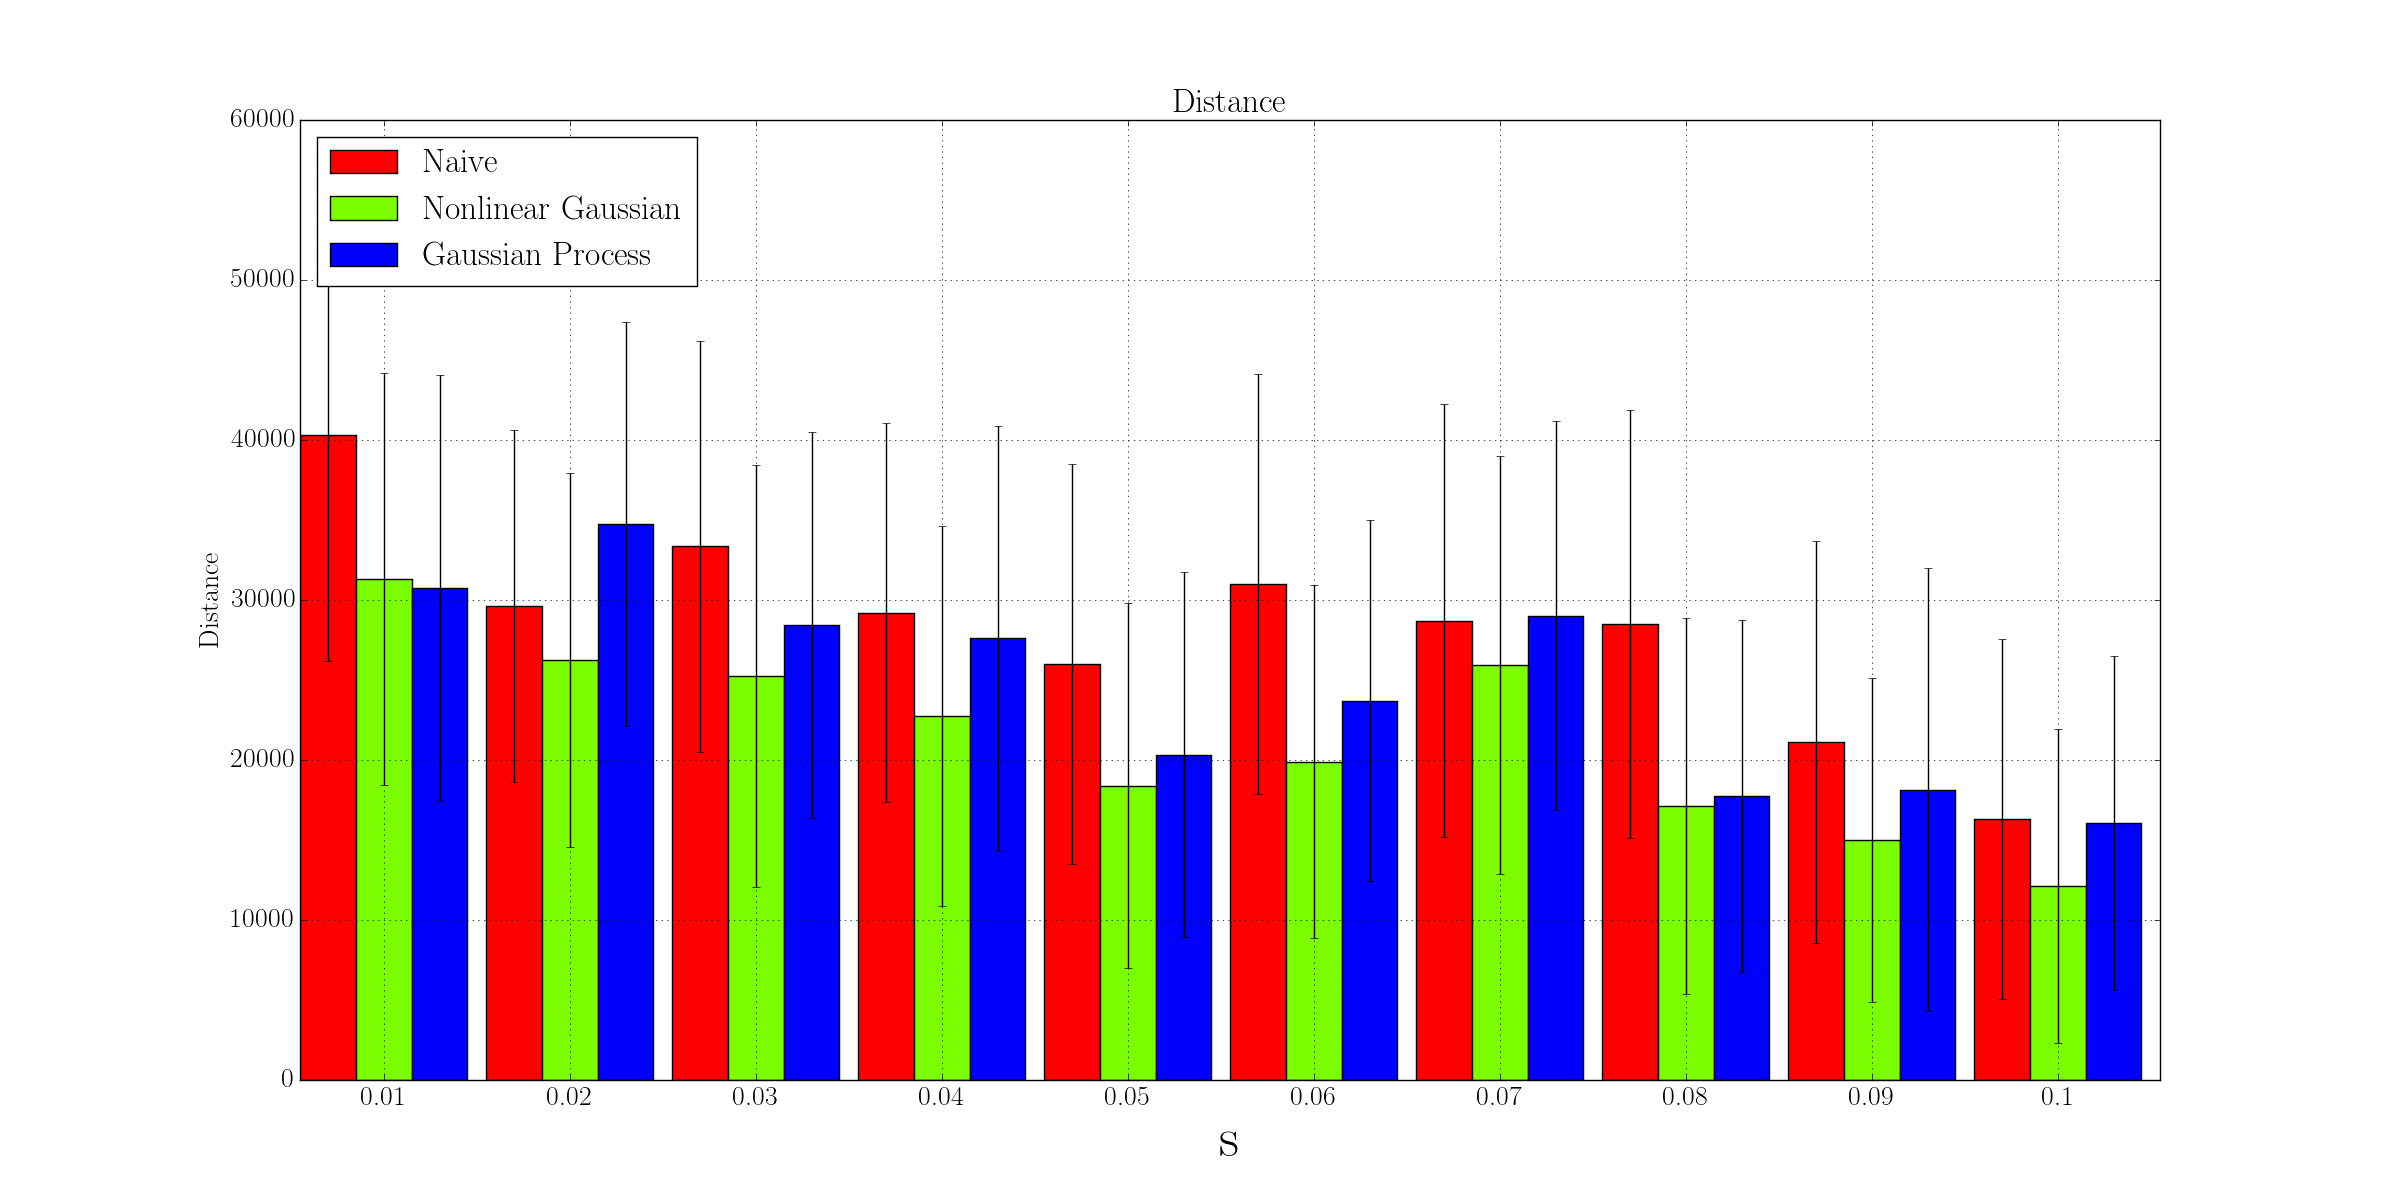
\includegraphics[width=\textwidth]{dist}
  \caption{Average distance to predicted site to the true site that is under selection.}
  \label{fig:Fig1}
\end{figure}

\paragraph{Rank}
\begin{figure}[H]
  \centering
    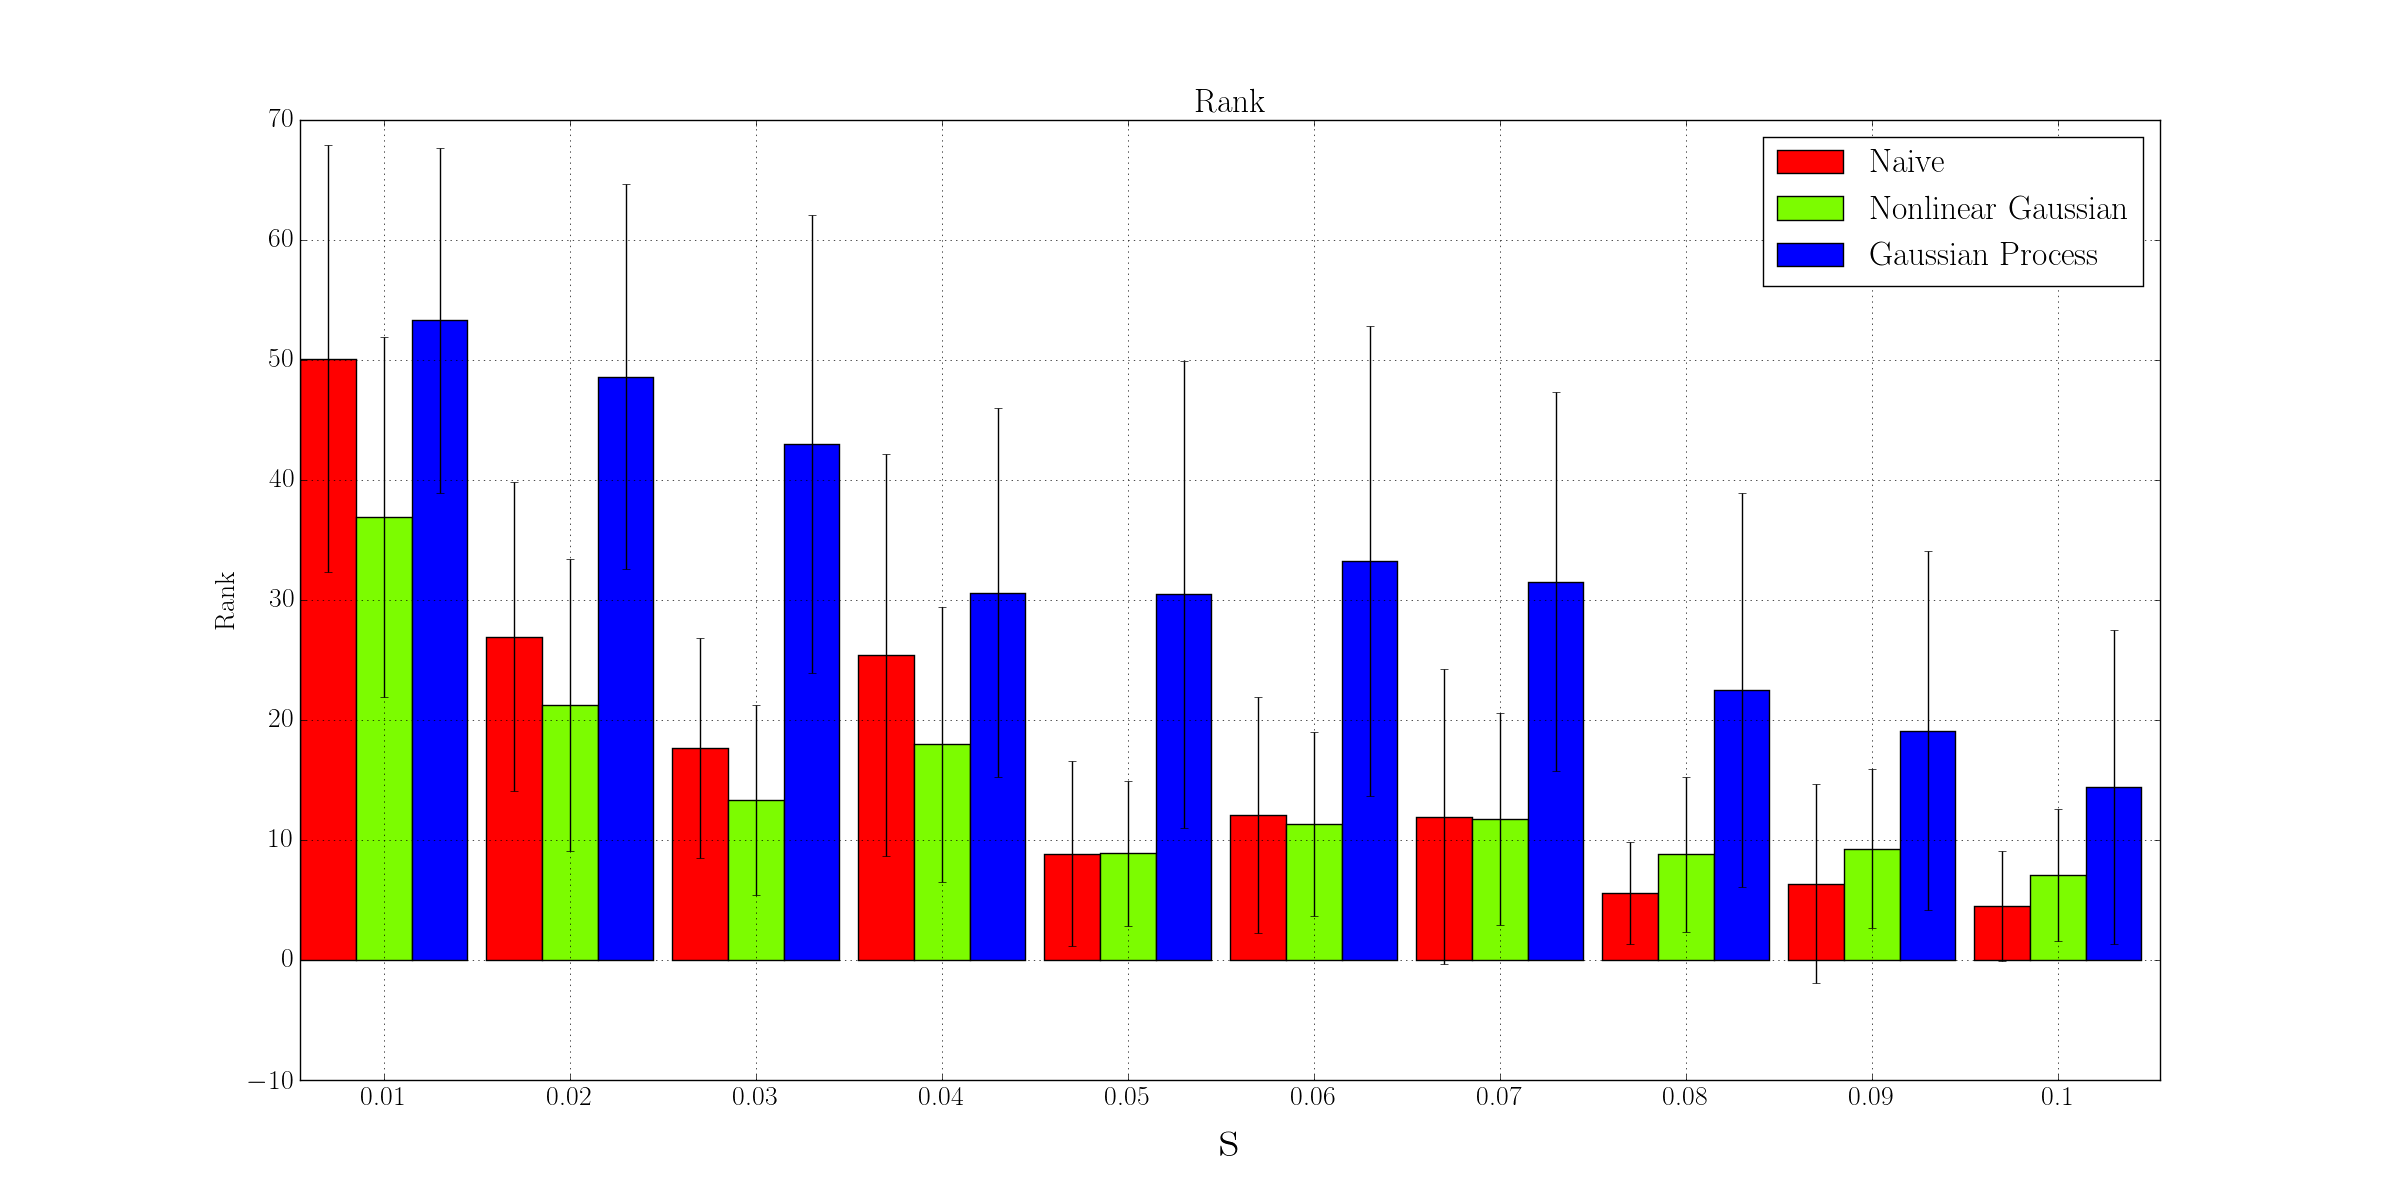
\includegraphics[width=\textwidth]{rank}
  \caption{Rank}
  \label{fig:Fig3}
\end{figure}

\paragraph{Mean Reciprocal Rank(MRR)}
\begin{figure}[H]
  \centering
    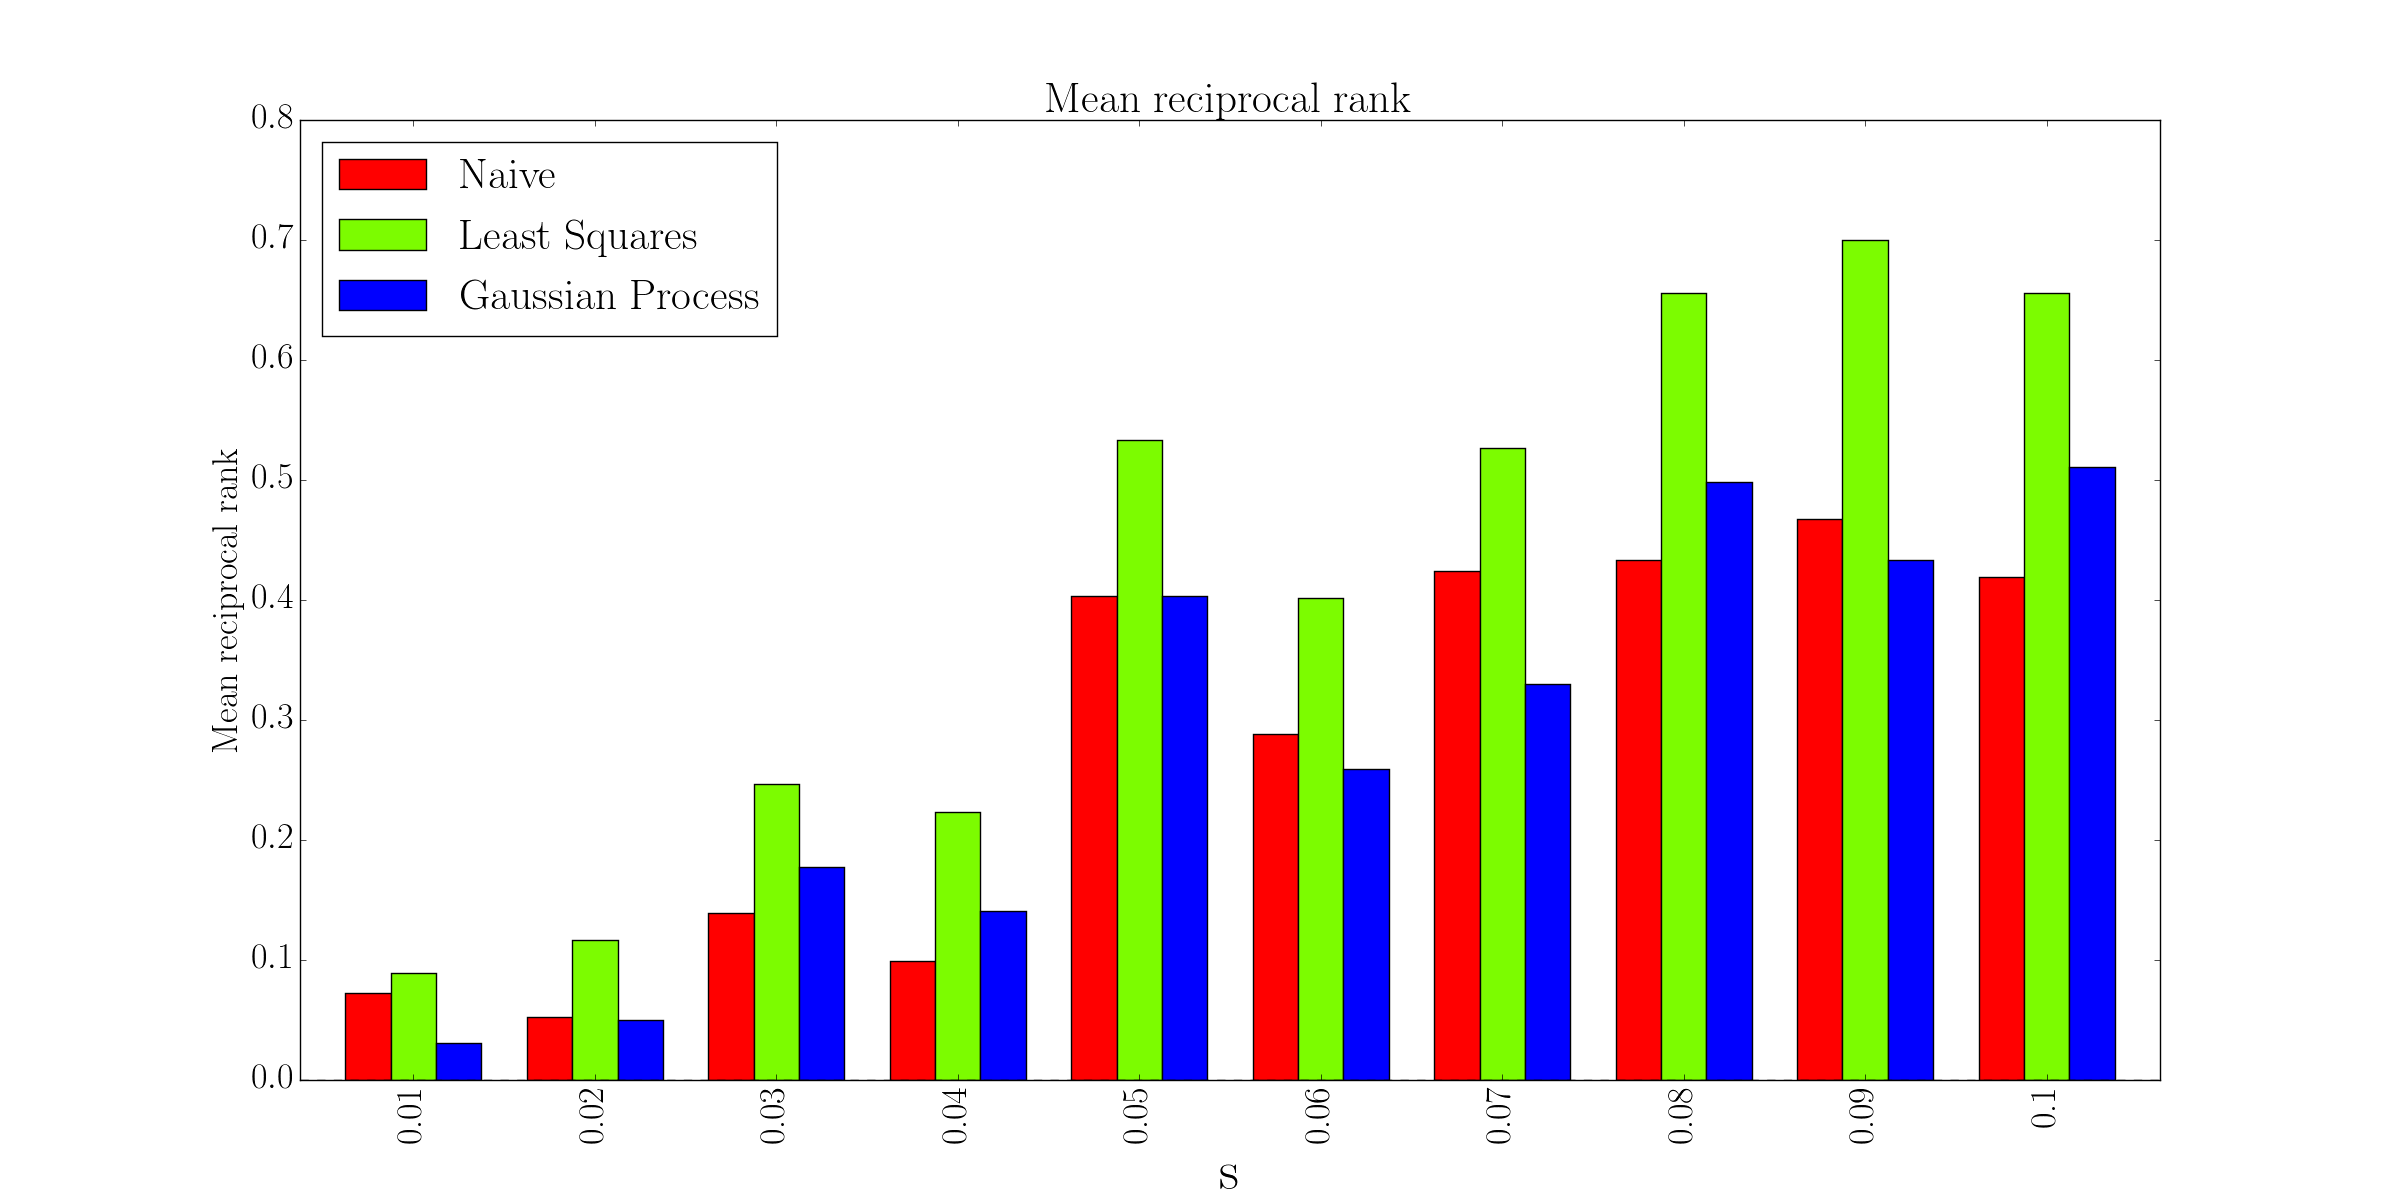
\includegraphics[width=\textwidth]{mrr}
  \caption{Mean Reciprocal}
  \label{fig:Fig2}
\end{figure}


\paragraph{Mean Average Precision (MAP)}
\begin{figure}[hh]
  \centering
    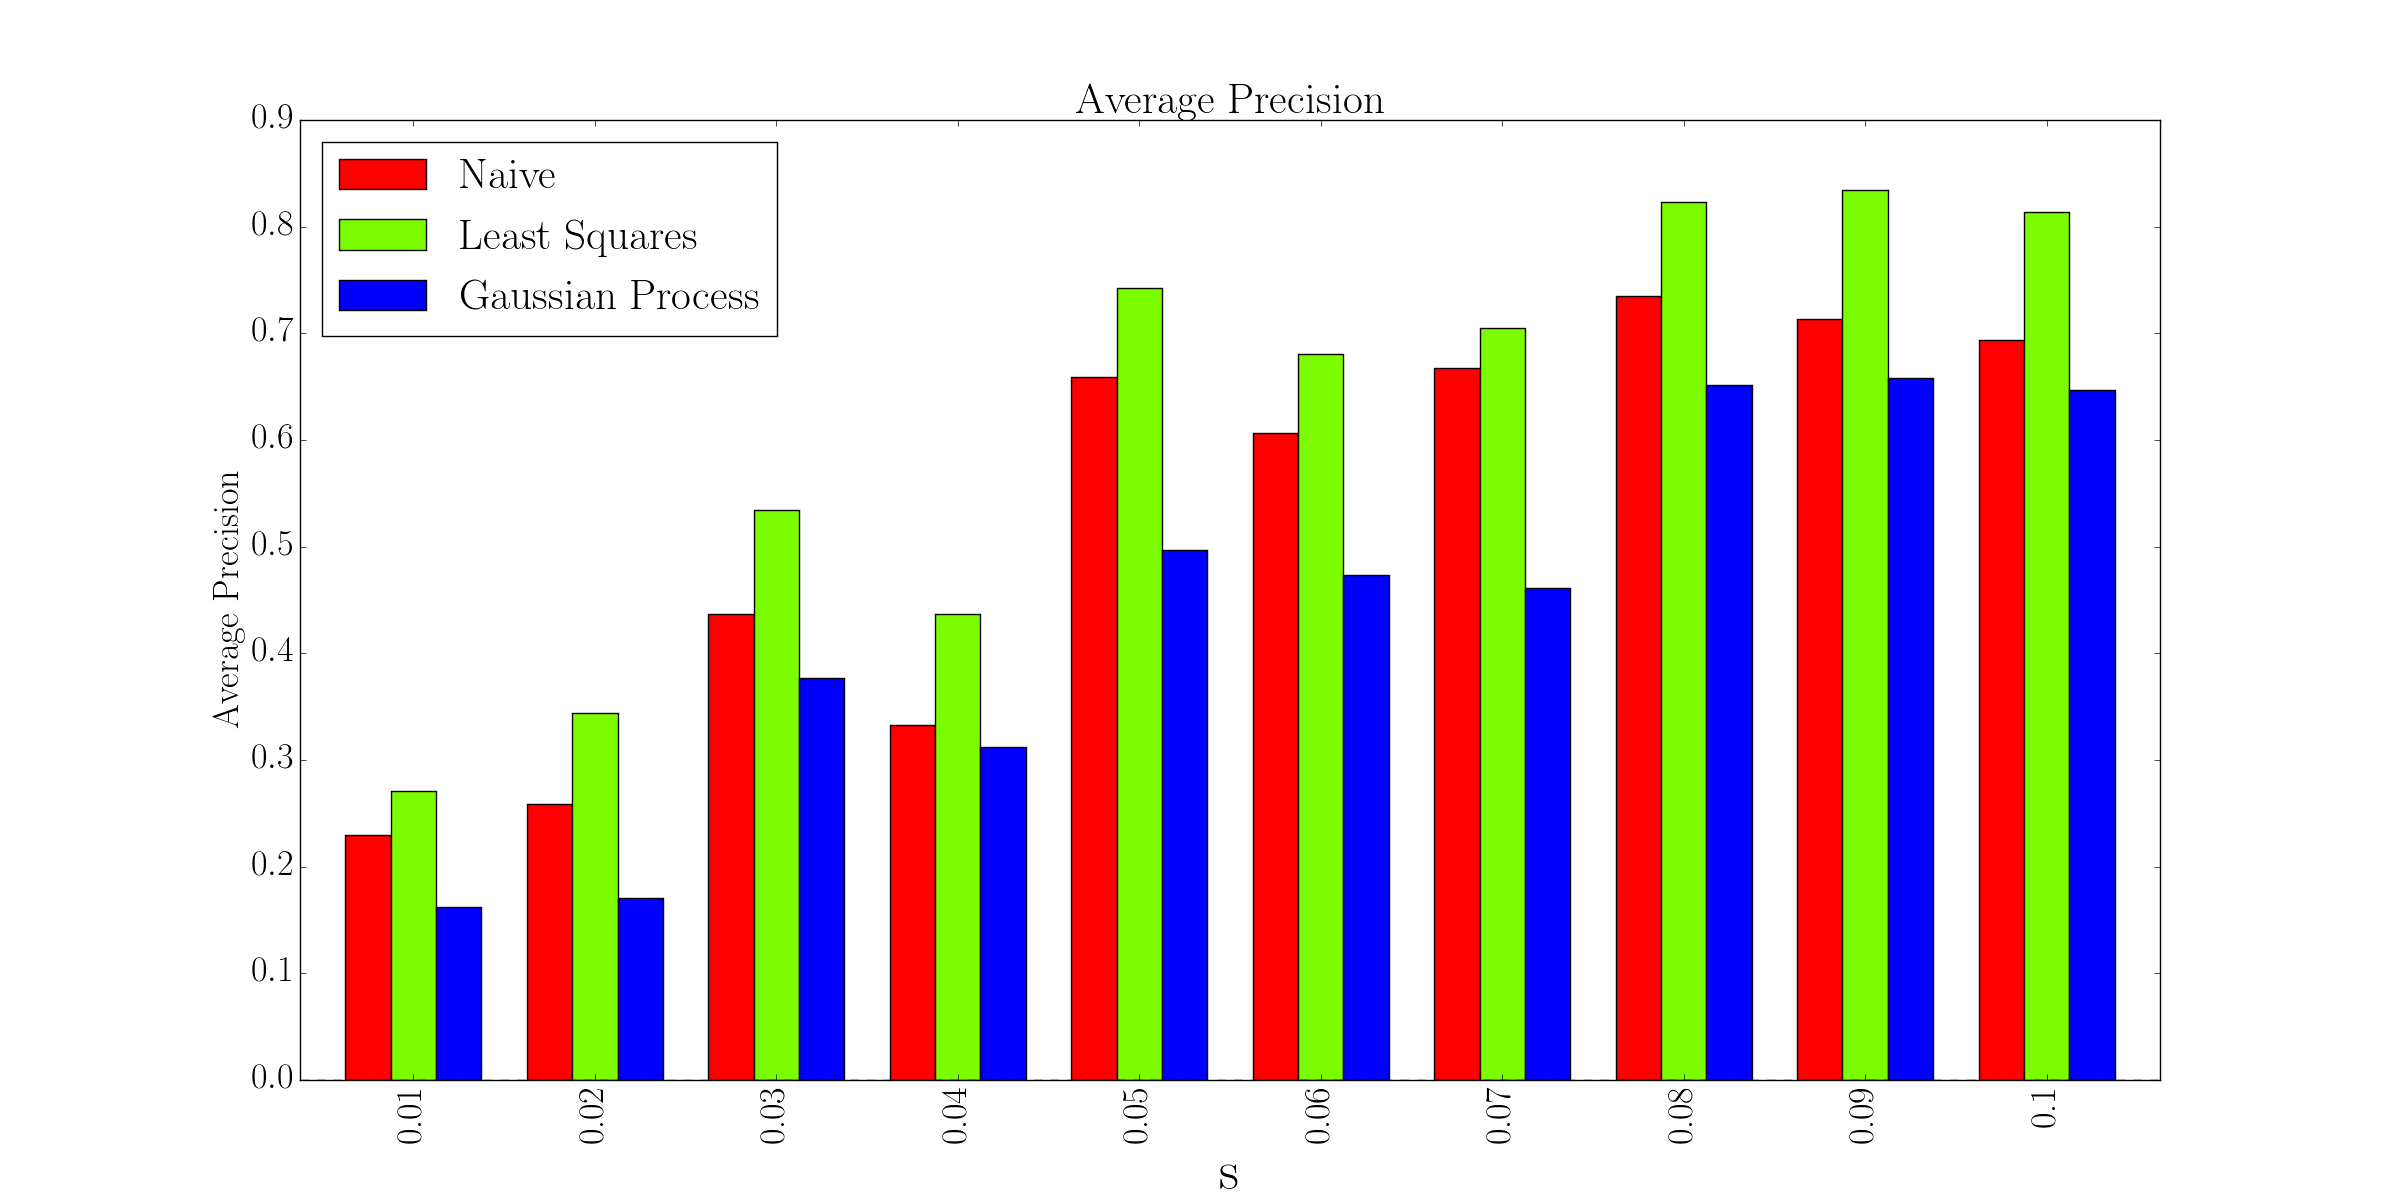
\includegraphics[width=\textwidth]{ap}
  \caption{Mean Average Precision (MAP)}
  \label{fig:Fig5}
\end{figure}


\subsubsection{Estimating Strength of Selection}
\begin{figure}[H]
  \centering
    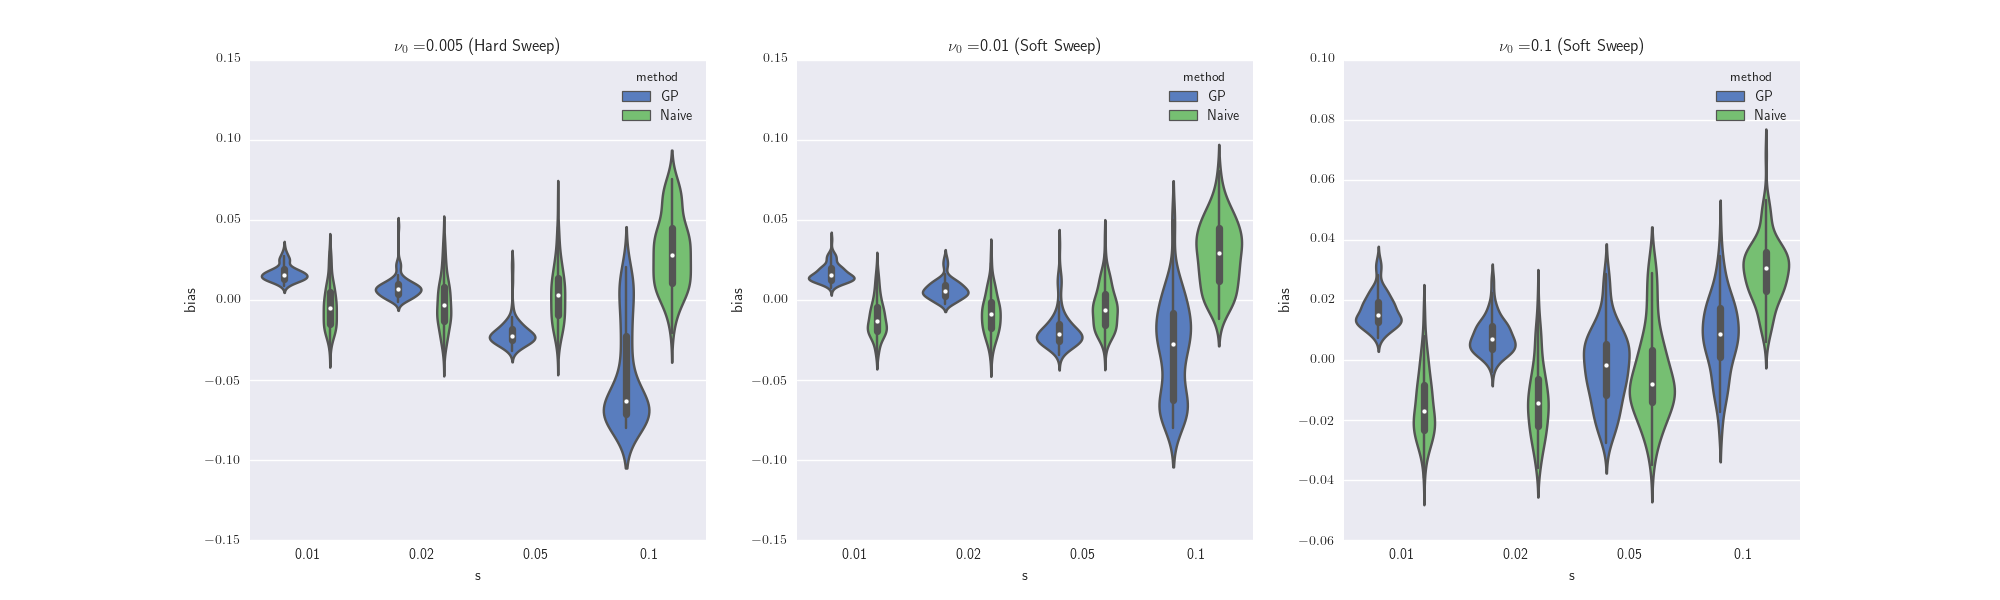
\includegraphics[width=\textwidth]{bias}
  \caption{Bias}
  \label{fig:Fig4}
\end{figure}

\subsection{Computational Performance}
\section{Discussions}


\bibliographystyle{plain}
\bibliography{library}

\end{document}